%\documentclass{PPFIT} % pro psaní v angličtině / for writing in English
\documentclass[czech]{PPFIT} % pro psaní v češtině / for writing in Czech
%\documentclass[slovak]{PPFIT} % pro psaní ve slovenštině / for writing in Slovak

%--------------------------------------------------------
%--------------------------------------------------------
%	PŘIZPŮSOBENÍ PDF / PDF CUSTOMIZATION
%--------------------------------------------------------

\hypersetup{
	pdftitle={Paper Title},
	pdfauthor={Author},
	pdfkeywords={Keyword1, Keyword2, Keyword3}
}

%--------------------------------------------------------
%--------------------------------------------------------
%  PŘEDBĚŽNÁ vs. KONEČNÁ VERZE / REVIEW vs. FINAL VERSION
%--------------------------------------------------------
%   NECHTE následující řádek zakomentovaný pro PŘEDBĚŽNÉ VERZE
%   Pro KONEČNOU VERZI řádek odkomentujte.
%   LEAVE this line commented out for the REVIEW VERSIONS
%   UNCOMMENT this line to get the FINAL VERSION

%\PPFinalCopy


\PPYear{2021/2022}

\ifczechslovak%
    %--------------------------------------------------------
    %--------------------------------------------------------
    %	INFORMACE O ČLÁNKU
    %--------------------------------------------------------    

  \PaperTitle{Metody Actor Critic pro spojitá prostředí}
	
	\Authors{Martin Kostelník, Michal Glos, Michal Szymik}
% 	\affiliation{*%
% 	  \href{mailto:herout@fit.vut.cz}{herout@fit.vut.cz},
% 	  \textit{Fakulta informačních technologií, Vysoké učení technické v Brně}}

	\Keywords{Klíčové slovo1 --- Klíčové slovo2 --- Klíčové slovo3}
	
	\Supplementary{\href{https://github.com/HrabaThor/KokosNET}{Github projektu}}

    %--------------------------------------------------------
    %--------------------------------------------------------
    %	ABSTRAKT
    %--------------------------------------------------------
    \Abstract{
        O jaký problém se jedná? O jaké téma? Jaký je cíl této práce?
        %	
        Jak se tento problém řeší a jak je cíle dosaženo (metodika)?
        \phony{Lorem ipsum dolor sit amet, consectetur adipiscing elit. Fusce ullamcorper suscipit euismod. Mauris sed lectus non massa molestie congue. In hac habitasse platea dictumst. Curabitur massa neque, commodo posuere fringilla ut, cursus at dui. Nulla quis purus a justo pellentesque.}
        %	
        Jaké jsou konkrétní výsledky? Jak dobře se daný problém řeší?
        \phony{Lorem ipsum dolor sit amet, consectetur adipiscing elit. Fusce ullamcorper suscipit euismod. Mauris sed lectus non massa molestie congue. In hac habitasse platea dictumst.}
        %	
        Takže co? Jak užitečná je tato práce pro vědu a pro čtenáře?
        \phony{Lorem ipsum dolor sit amet, consectetur adipiscing elit. Fusce ullamcorper suscipit euismod.}
    }
\else%
  
\fi

%--------------------------------------------------------
%--------------------------------------------------------
%	TEASER 
%--------------------------------------------------------
\Teaser{
%	\TeaserImage{placeholder.pdf}
%	\TeaserImage{placeholder.pdf}
%	\TeaserImage{placeholder.pdf}
}

%--------------------------------------------------------
%--------------------------------------------------------
%--------------------------------------------------------
%--------------------------------------------------------
\begin{document}
\startdocument
%--------------------------------------------------------
%--------------------------------------------------------
%	OBSAH ČLÁNKU / CONTENT OF THE ARTICLE
%--------------------------------------------------------
\ifczechslovak
    \section{Úvod}

% MOTIVACE
Cílem tohoto projektu bylo vytvořit vlastní implementaci algoritmů posilovaného učení (RL), především Actor-Critic pro spojitá prostředí. Jsou využity prostředí knihoven OpenaI Gym\footnote{\url{https://www.gymlibrary.ml/}} a dm\_control \cite{tunyasuvunakool2020}. S výslednou implementací je prováděno několik sad experimentů, které demonstrují úspěšnost implementace.

% DEFINICE PROBLÉMU
Prováděné experimenty srovnávají úspěšnost naší implementace s algoritmy z knihovny stable-baselines-3\footnote{\url{https://stable-baselines3.readthedocs.io/en/master/index.html}} která obsahuje řadu různých implementací algoritmů posilovaného učení. Během experimentů se zkoumá vliv jednotlivých parametrů na celkovou úspěšnost agenta, jako je architektura neuronových sítí, nastavení aktivačních funkcí a obecně různé nastavení parametrů specifických pro typ implementované metody. 

% EXISTUJÍCÍ ŘEŠENÍ
V tomto projektu se zabýváme implementací TD3 algoritmu (viz \ref{sec:TD3}), který vychází z jiného Actor-Critic algoritmu Deep Deterministic Policy Gradient Agents (DDPG), do kterého přináší několik změn aby nedocházelo k přeceňování value funkce.

\section{Actor-critic a algoritmus TD3}
\label{sec:TD3}
Metody actor-critic jsou specifické tím, že mají oddělenou strukturu pro policy a value funkci. Policy síť se nazývá actor a síť aproximující value funkci se nazývá critic. Úkolem sítě actor je vybírat akce, které mu poté critic kritizuje, čili aproximuje očekávanou value funkci. Průběh učení agenta je dobře vidět na diagramu v obrázku \ref{fig:ac_diagram}.

\begin{figure}[t]
	\centering
	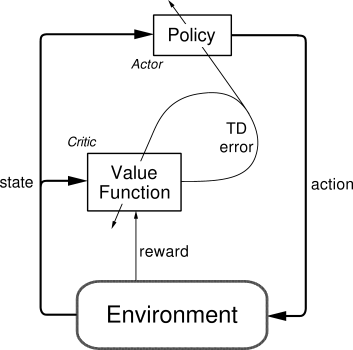
\includegraphics[width=0.7\linewidth]{ac_diagram.png}
	\caption{Diagram znázorňující průběh učení agenta používajícího actor-critic metodu.}
	\label{fig:ac_diagram}
\end{figure}

Twin-delayed deep deterministic policy gradient (TD3) je jedním z actor-critic algoritmů. Jedná se o online a off-policy učící metodu, založenou na principu actor-critic. TD3 agent hledá takovou optimální policy, která maximalizuje očekávanou kumulovanou odměnu. Agent používá dvě critic sítě, kterými se učí dvě value funkce a pro aktualizaci policy používá minimální odhad value funkce. Policy se updatuje méně často než Q-funkce a během její aktualizace se přidává šum k vybrané akci, tudíž se na základě policy budou s menší pravděpodobností vybírat akce s vysokým odhadem value.
\cite{TD3MathWorks}
%--------------------------------------------------------
%--------------------------------------------------------
%--------------------------------------------------------
%--------------------------------------------------------
\section{Popis řešení}
\label{sec:IMplementation}
Projekt je implementován v jazyce Python3 s použitím knihoven \texttt{Gym}, \texttt{MuJoCo} \cite{todorov2012mujoco},\\\texttt{stable\_baselines3} a několika dalších podpůrných nástrojů.

\subsection{Implementace TD3}
Agenta lze spustit ve dvou módech: trénovacím a evaluačním. Při evaluačním módu se načte již existující a natrénovaný model a provede se několik běhů v daném prostředí. Z běhů je vypočtena průměrná odměna, která je vytištěna na standardní výstup. Součástí evaluace je taky vykreslování chování agenta do okna a vytvoření videa.

Zajímavější je trénování. Po nastavení všech parametrů uživatelem je vytvořeno celkem šest neuronových sítí. Dvě pro síť actor (actor a actor-target) a dvě pro každou ze dvou sítí critic (critic1,2 a critic1,2-target). Také se provede naplnění paměti agenta náhodnými akcemi v náhodných stavech prostředí s příslušnými odměnami. V tuto chvíli můžeme začít samotné trénování. To trvá daný počet kroků a v každém z nich provedeme akci vybranou sítí actor, ke které je přidán šum.

Také provedeme optimalizační akci, ve které se náhodně vybere několik vzpomínek z paměti. Vypočítáme hodnotu value funkce pro obě critic-target sítě vybereme z nich menší hodnotu a s pomocí chybové funkce MSE spočítáme loss sítí critic.

Optimalizace sítě actor se provádí pouze co N kroků. Zde nám stačí pro dané stavy z paměti vygenerovat akce a jako chybu vzít negativní průměr hodnot daných sítí critic. Na konci trénovacího kroku se provede aktualizace target sítí tak, že se provede lineární kombinace parametrů s non-target sítí s využitím parametru $\tau \in <0, 1>$. 


\section{Experimenty}
%--------------------------------------------------------
%--------------------------------------------------------
Pro vyhodnocení výsledného implementovaného algoritmu jsme se rozhodli provést řadu experimentů. V první sadě experimentů jsme prováděli porovnání našeho TD3 algoritmu s existující implementací z knihovny stable-baselines-3\footnote{\url{https://stable-baselines3.readthedocs.io/en/master/modules/td3.html}}. Využili jsme méně komplexních prostředí fyzikálního simulátoru MuJoCo\footnote{\url{https://mujoco.org/}}. Druhá sada experimentů se zabývá vlivem nastavení hyperparametrů na agentovo učení v prostředí Hopper.


\subsection{Srovnání se stable-baselines-3}

\begin{figure*}[ht]\centering % Využití \begin{figure*} způsobí roztažení obrázku na celou šířku stránky
  \centering
  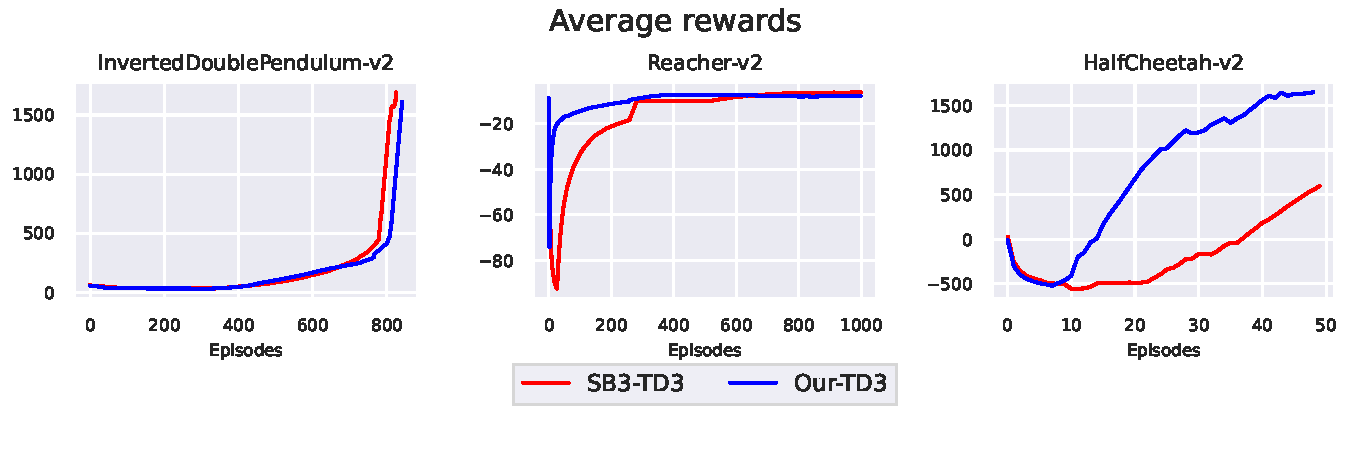
\includegraphics[width=\linewidth]{images/comparison_all.pdf}\\[1pt]
  \caption{Srovnání průběhu učení agenta pro naši implementaci a pro implementaci ze stable-baselines-3.}
  \label{fig:srovnani}
\end{figure*}

Pro porovnání našeho algoritmu s existující implementací z knihovny stable-baselines-3 jsme si vybrali tři prostředí z MuJoCo:\\ \texttt{InvertedDoublePendulum-v2}, \texttt{Reacher-v2} a \texttt{HalfCheetah-v2}. Pro vyhodnocení jsme použili kritérium průměrné odměny z posledních 256 epizod. Pro každé prostředí byly nastaveny stejné hyperparametry u obou implementací. Výsledky učení pro 50000 časových kroků v každém prostředí lze vidět na obrázku \ref{fig:srovnani}.

Nejlepší natrénované modely obou algoritmů byly evaluovány na 1000 epizodách. Výsledky evaluace jsou v tabulce \ref{tab:srovnani_evaluace}, která ukazuje průměrnou hodnotu odměň přes všechny provedené epizody.

\begin{table}[h]
% 	\vskip6pt
	\centering
	\begin{tabular}{| l | c | c | c | }
% 		\hline
% 		& \multicolumn{3}{c|}{Prostředí} \\
		\hline
	    
		& Inverted & & \\
		& Double & Reacher & HalfCheetah\\
		& Pendulum & & \\
		\hline
		Our-TD3 & $9349.20$ & $-6.08$ & $2856.33$ \\
        \hline
		SB3-TD3 & $4140.74$ & $-4.84$ & $2493.56$ \\
		\hline
	\end{tabular}
	\caption{Průměrné hodnoty odměn při evaluaci algoritmů na 1000 epizodách.}
	\label{tab:srovnani_evaluace}
\end{table}


Výsledky tohoto experimentu naplňují očekávání. Náš algoritmus se učí řešit prostředí s velice podobnými výsledky jako existující stable-baseline-3 implementace. Pro úplné porovnání by bylo třeba provést více experimentů s různým nastavením hyperparametrů, výše uvedené porovnání nám ale přišlo pro účely tohoto projektu dostatečné.

%--------------------------------------------------------
%--------------------------------------------------------
\subsection{Nastavení hyperparametrů}
    Druhá sada experimentů se snaží zjistit závislost úspěšnosti agenta na nastavení hyperparametrů. Všechny experimenty budeme provádět v prostředí \texttt{Hopper-v2} a budeme sledovat průměr odměn z posledních 256 kroků a chybové funkce obou sítí.
    
    Budeme sledovat efekt discount factoru $\gamma$, kombinačního parametru $\tau$, různé architektury sítí a různá nastavení frekvence učení sítě actor. Tyto všechny výsledky budeme porovnávat s výchozím nastavením parametrů, které je následující:
    
    \begin{itemize}
        \item $gamma = 0.99$
        \item $\tau = 0.005$
        \item $net = \{400, 300\}$
        \item $delay = 2$
    \end{itemize}
    
    Budeme vždy trénovat na 200000 kroků a budeme testovat následující možnosti parametrů:
    
    \begin{itemize}
        \item $gamma \in \{0.0, 0.5, 0.9, 1.0\}$
        \item $\tau \in \{0.0, 0.05, 0.1, 0.4, 0.8, 1.0\}$
        \item $net \in \{\{64, 64, 64\}, \{512, 256, 128\}\}$ a různé velikosti sítí actor a critic
        \item $delay \in \{1, 4, 10\}$
    \end{itemize}
    
    Výsledky experimentů můžeme vidět na obrázcích na konci tohoto dokumentu počínaje obrázkem \ref{fig:default}. Můžeme si všimnout, že i při dlouhém tréningu nenastalo zlepšení, ale agent se nejlépe choval už po méně než 5000 epizodách. Parametr $\gamma$ je nejlepší nechat co nejvyšší, velice blízký hodnotě $1.0$. Zdá se, že architektury jednotlivých sítí na výsledek neměly nějaký značný vliv a všechny experimenty se chovaly velice podobně.
    
    Frekvence provádění optimalizace sítě actor je lepší ponechat na nižších hodnotách, experimentálně dopadl nejlépe výchozí parametr s hodnotou $2$. U parametru $\tau$ se jeví nejlepší ponechat ho velice blízko nule, zajímavého výsledku si můžeme všimnou na obrázku \ref{fig:boom}, kde se dlouho nic nedělo a ke konci učení odměny explodovaly. Při vyšších nastaveních se agent neučí vůbec.
%--------------------------------------------------------
%--------------------------------------------------------


%--------------------------------------------------------
%--------------------------------------------------------



\section{Závěr}
\label{sec:Conclusions}

Hlavní náplní této práce bylo naprogramovat vlastní implementaci actor-critic algoritmu. Vytvořený algoritmus svými specifiky odpovídá metodě TD3 a je schopný řešit úlohy z prostředí MuJoCo. Učení agenta používajícího náš algoritmus dosahuje dobrých výsledků a je velice podobné učení agenta používajícího existující implementaci TD3 ze stable-baselines-3. 

Dále jsme v této práci ukázali, že je možné v naší implementaci nastavovat různé hyperparametry jednotlivých komponent algoritmu, což jsme následně demonstrovali na několika experimentech, které ukazují vliv hyperparametrů na učení agenta.

Porovnání průběhu učení agenta s existující implementací proběhlo na třech MuJoCo prostředích a ve všech případech lze pozorovat velice podobný tvar křivky průměrných odměn. Lze tedy předpokládat, že náš algoritmus dosahuje podobné úrovně kvality jako již existující implementace.

Implementace našeho algoritmu umožňuje experimentování ať už na nejnižší úrovni se samotnou metodou TD3, tak na vyšší úrovni s trénováním agenta s různými hyperparametry na libovolných prostředích knihovny OpenAI Gym (tedy nejsou limitovány pouze na MuJoCo). Výsledky agentova učení lze porovnávat s jinými existujícími implementacemi.

\begin{figure*}[ht]
  \centering
  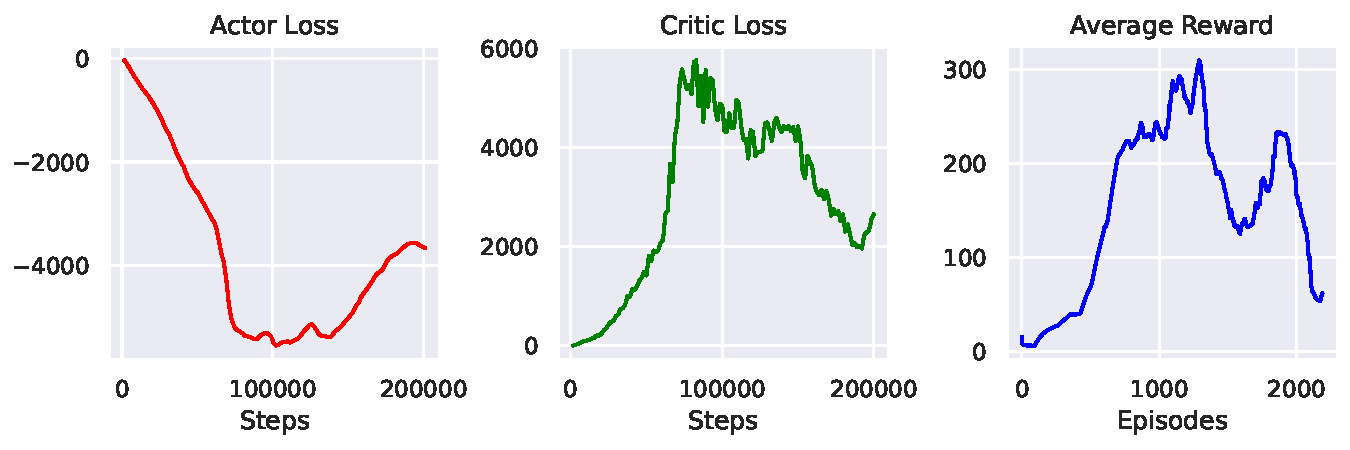
\includegraphics[width=\linewidth]{images/exp-hopper-default.pdf}
  \caption{Výchozí nastavení parametrů.}
  \label{fig:default}
\end{figure*}

\begin{figure*}[ht]
  \centering
  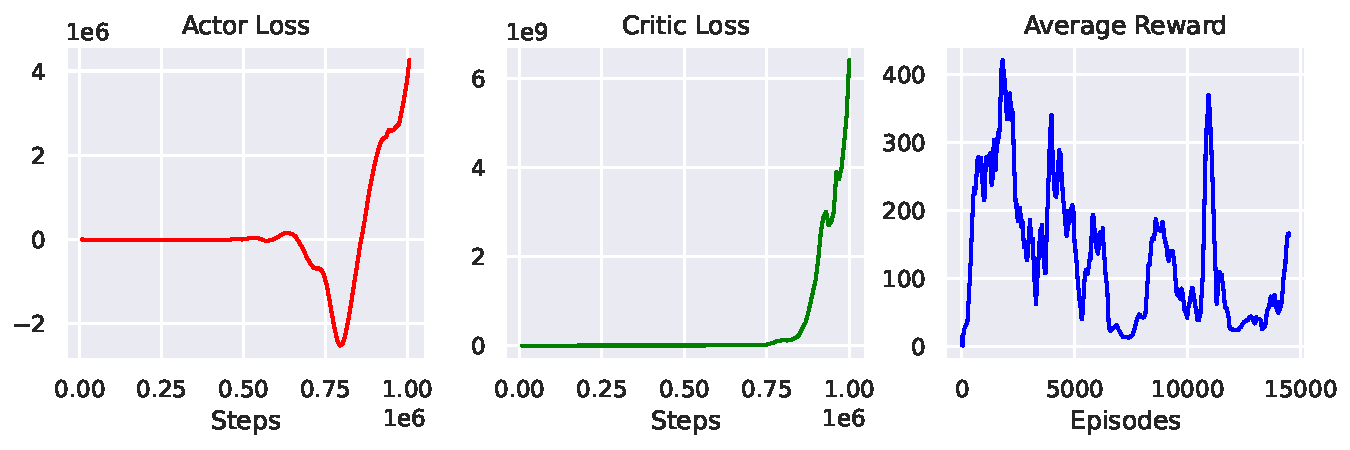
\includegraphics[width=\linewidth]{images/exp-hopper-1M.pdf}
  \caption{Výchozí parametry pro 1M kroků.}
\end{figure*}

\begin{figure*}[ht]
  \centering
  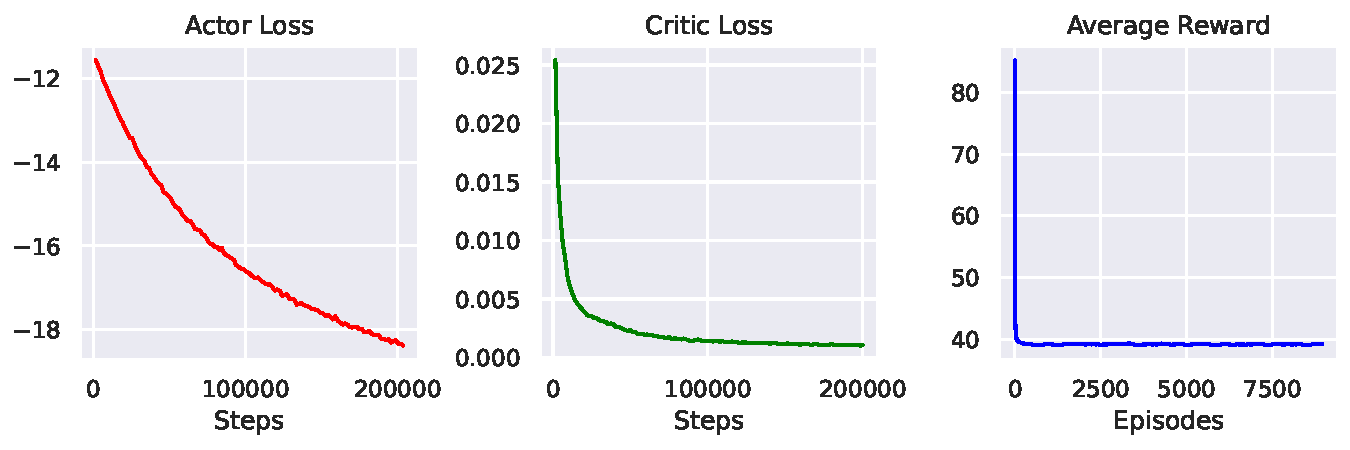
\includegraphics[width=\linewidth]{images/exp-gamma0.0.pdf}
  \caption{$\gamma=0.0$.}
\end{figure*}

\begin{figure*}[ht]
  \centering
  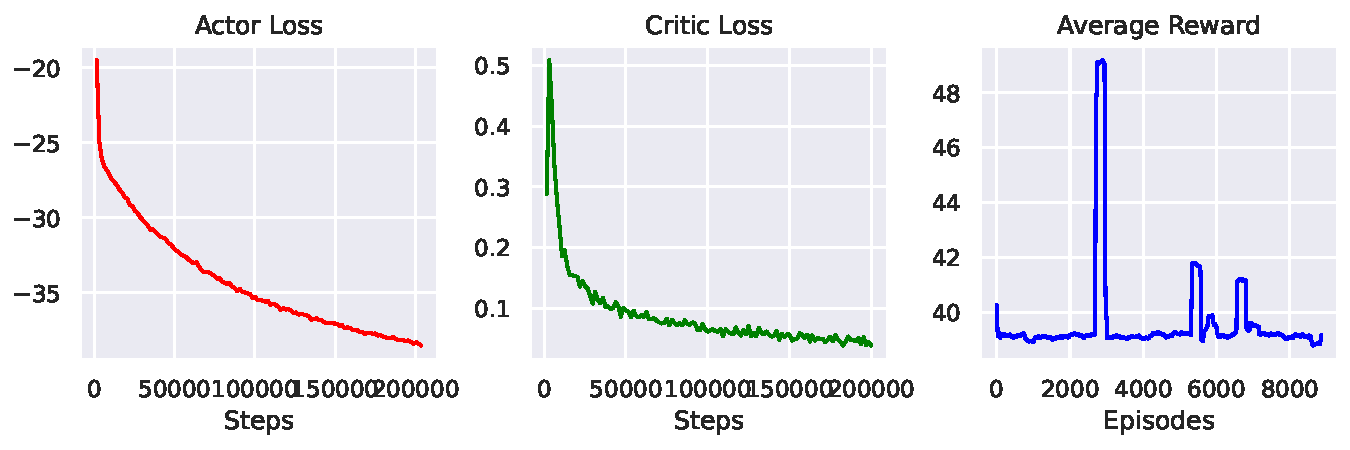
\includegraphics[width=\linewidth]{images/exp-gamma0.5.pdf}
  \caption{$\gamma=0.5$.}
\end{figure*}

\begin{figure*}[ht]
  \centering
  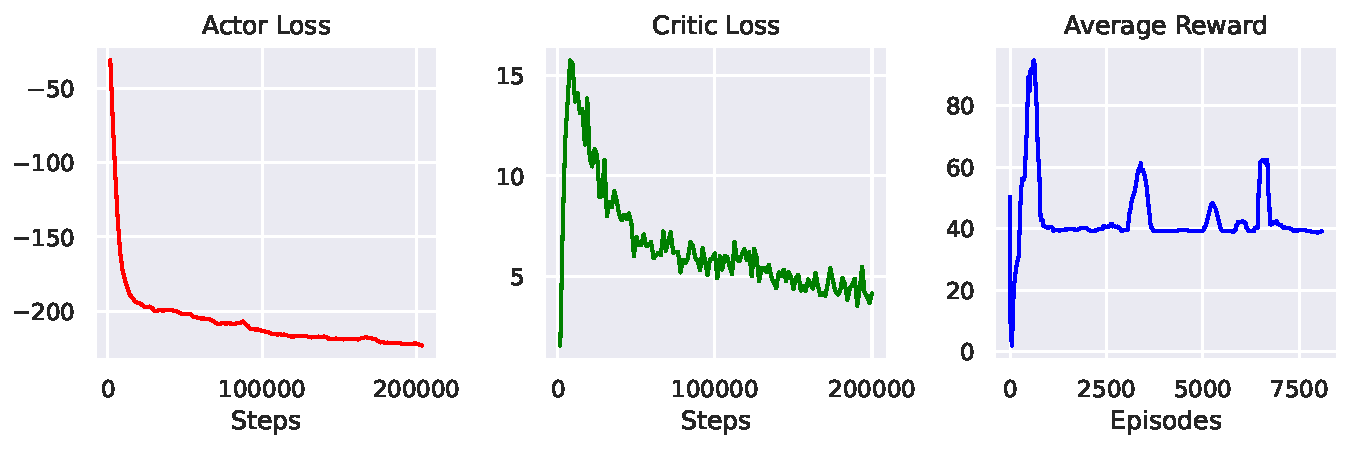
\includegraphics[width=\linewidth]{images/exp-gamma0.9.pdf}
  \caption{$\gamma=0.9$.}
\end{figure*}

\begin{figure*}[ht]
  \centering
  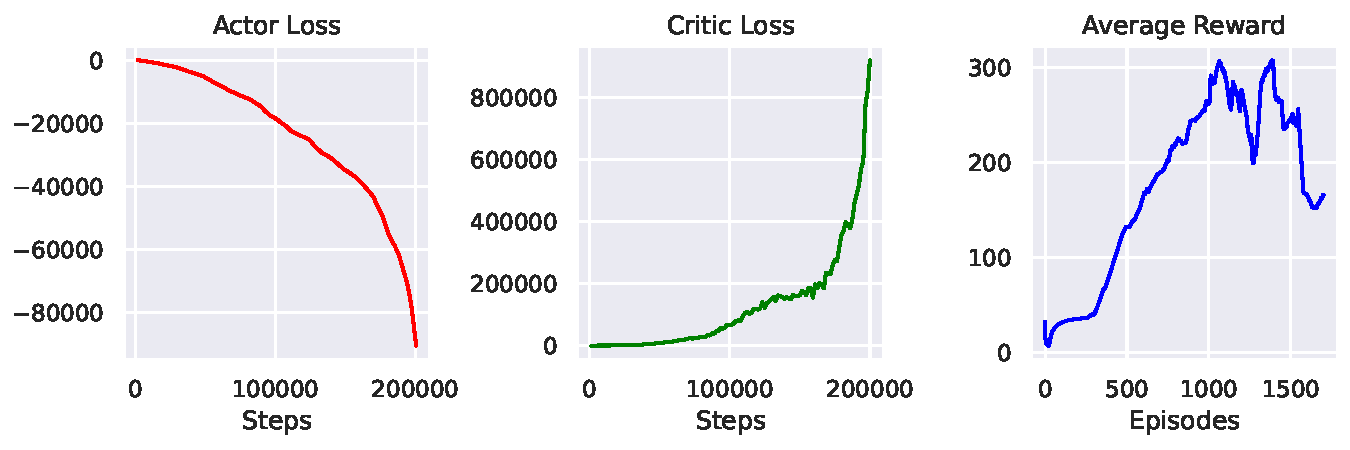
\includegraphics[width=\linewidth]{images/exp-gamma1.0.pdf}
  \caption{$\gamma=1.0$.}
\end{figure*}

\begin{figure*}[ht]
  \centering
  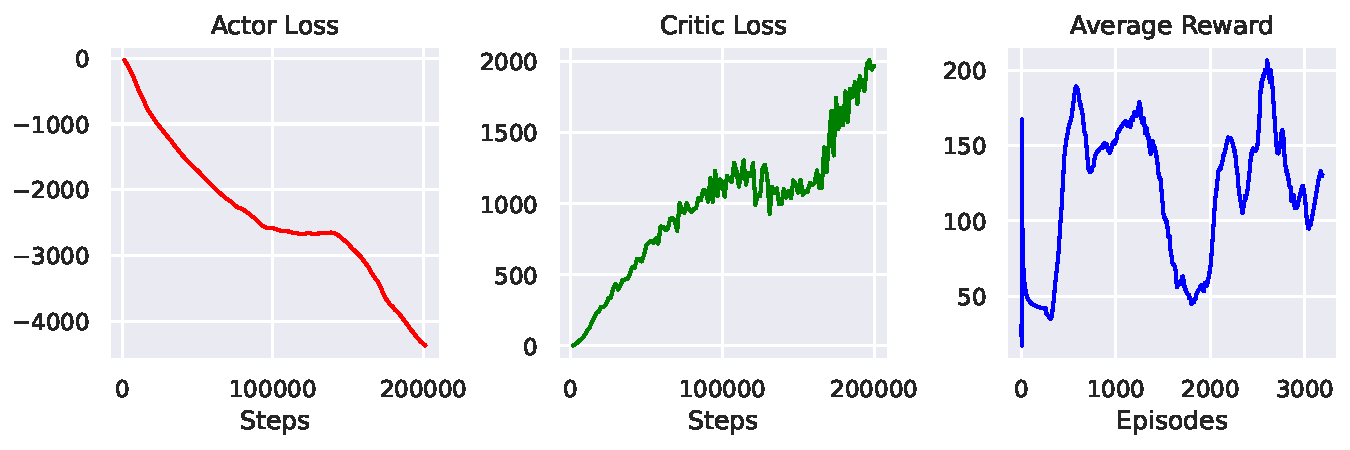
\includegraphics[width=\linewidth]{images/exp-hopper-64-64-64.pdf}
  \caption{$nets = \{64, 64, 64\}$.}
\end{figure*}

\begin{figure*}[ht]
  \centering
  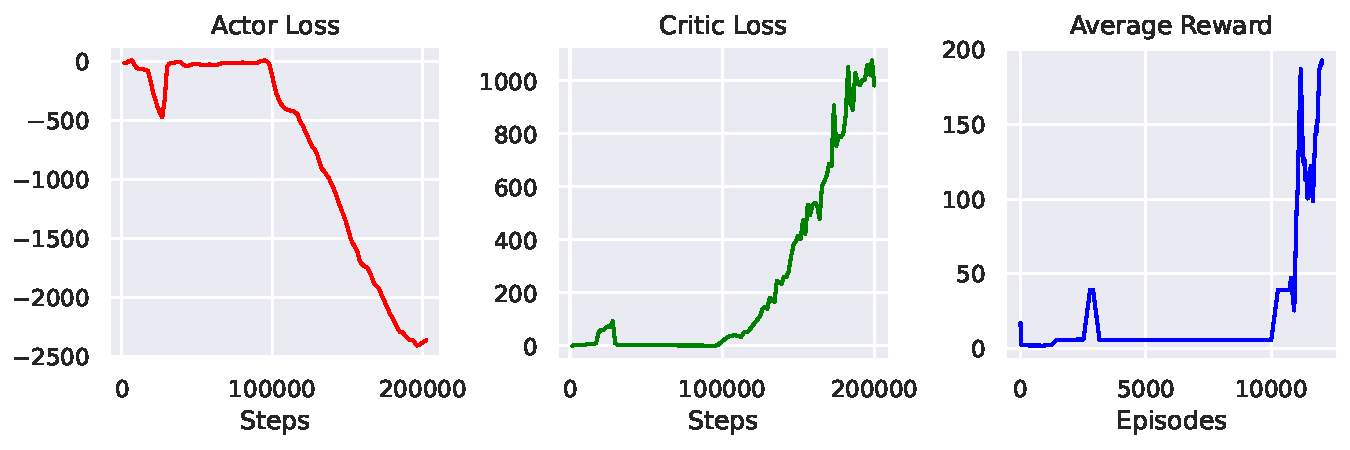
\includegraphics[width=\linewidth]{images/exp-hopper-512-256-128.pdf}
  \caption{$nets = \{512, 256, 128\}$.}
\end{figure*}

\begin{figure*}[ht]
  \centering
  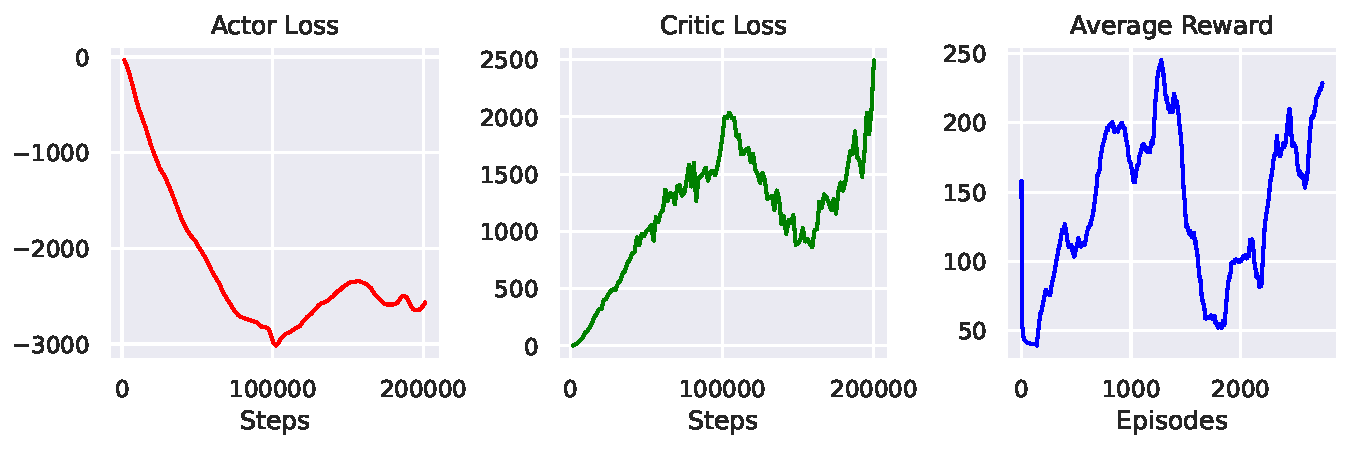
\includegraphics[width=\linewidth]{images/exp-hopper-Aless.pdf}
  \caption{$actor = \{256, 256\}, critic = \{256, 256, 256\}$.}
\end{figure*}

\begin{figure*}[ht]
  \centering
  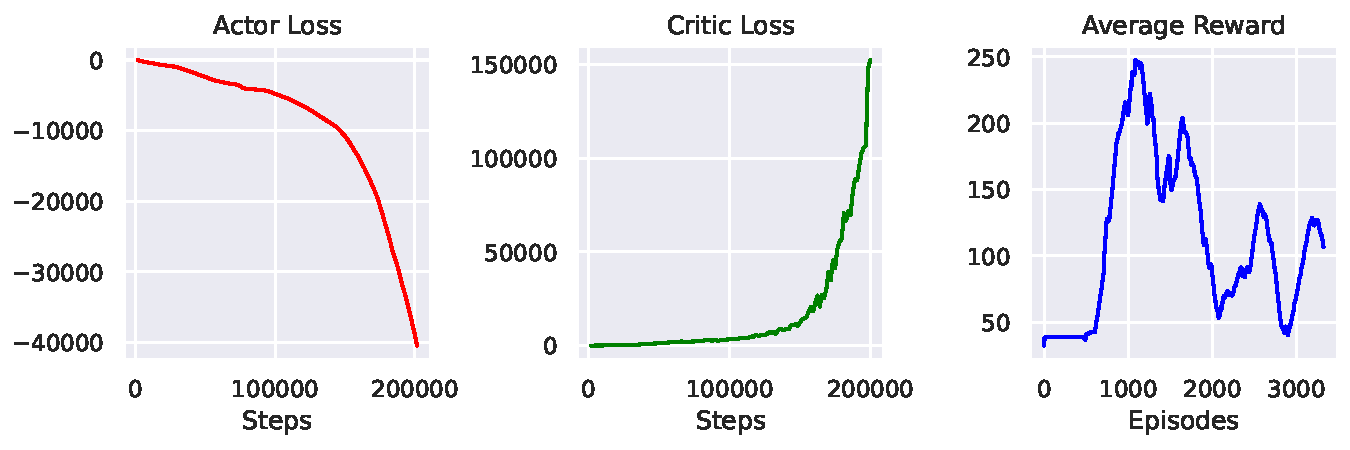
\includegraphics[width=\linewidth]{images/exp-hopper-Amore.pdf}
  \caption{$actor = \{256, 256, 256\}, critic = \{256, 256\}$.}
\end{figure*}

\begin{figure*}[ht]
  \centering
  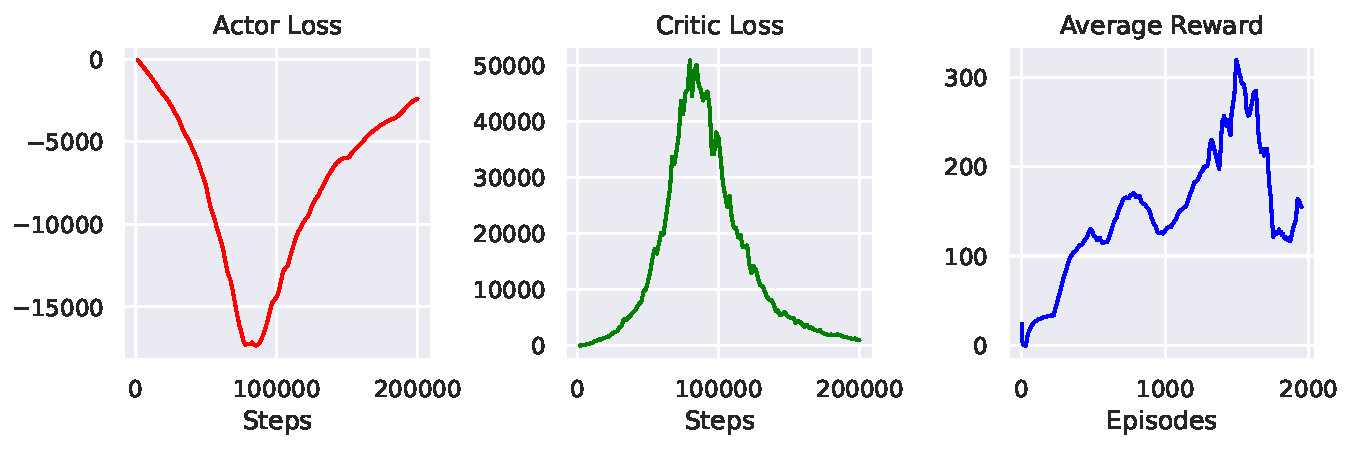
\includegraphics[width=\linewidth]{images/exp-hopper-policy1.pdf}
  \caption{$delay = 1$.}
\end{figure*}

\begin{figure*}[ht]
  \centering
  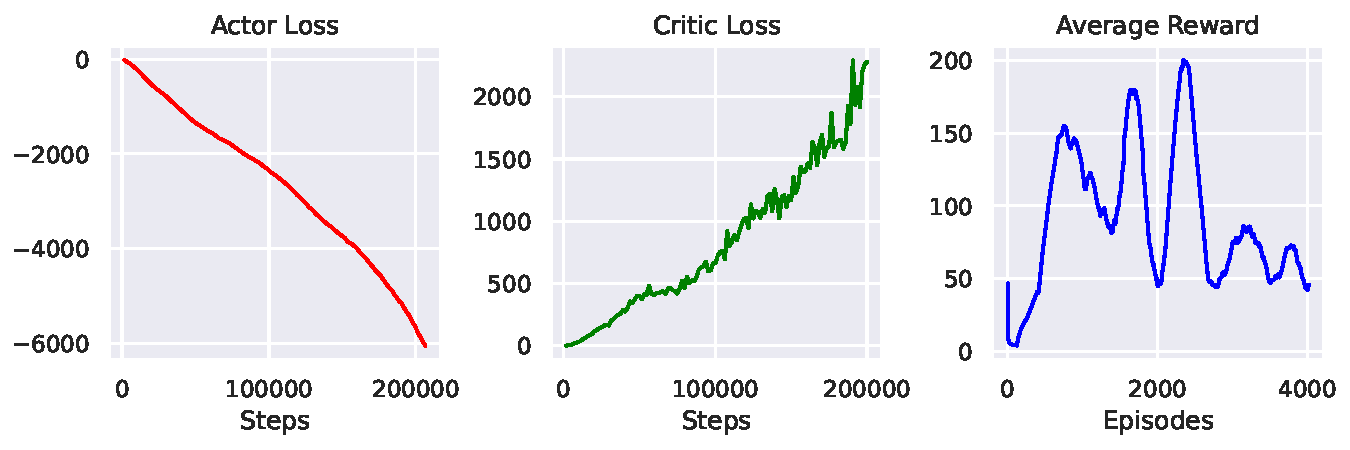
\includegraphics[width=\linewidth]{images/exp-hopper-policy4.pdf}
  \caption{$delay = 4$.}
\end{figure*}

\begin{figure*}[ht]
  \centering
  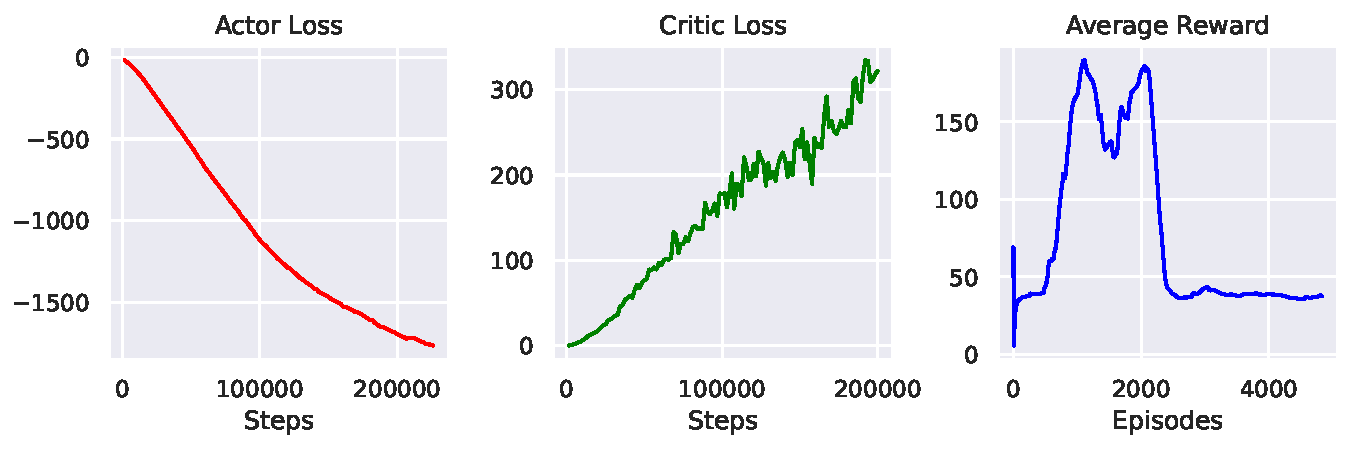
\includegraphics[width=\linewidth]{images/exp-hopper-policy10.pdf}
  \caption{$delay = 10$.}
\end{figure*}

\begin{figure*}[ht]
  \centering
  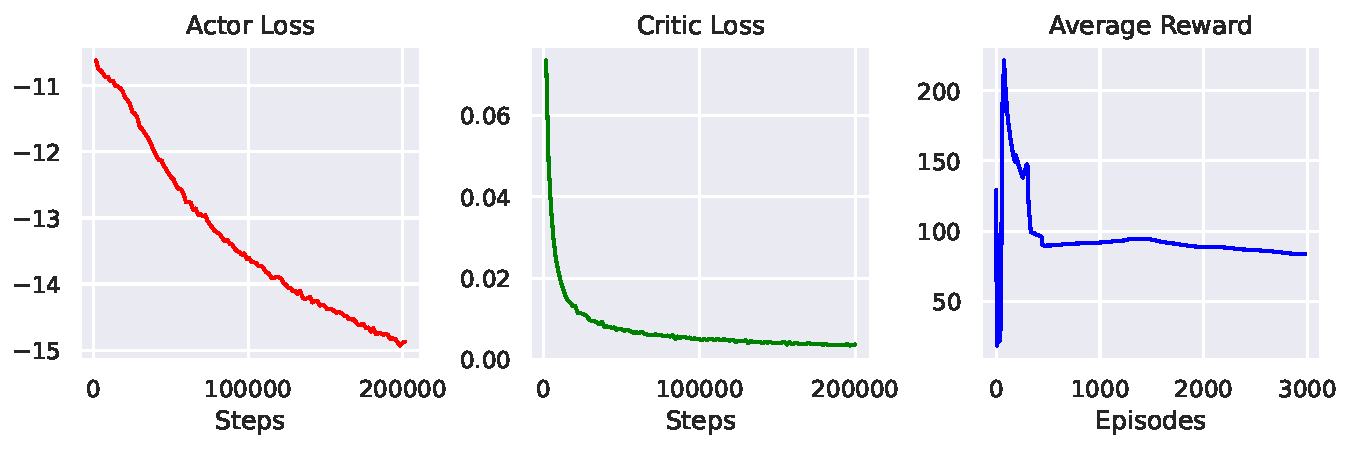
\includegraphics[width=\linewidth]{images/exp-hopper-tau0.0.pdf}
  \caption{$\tau = 0.0$.}
\end{figure*}

\begin{figure*}[ht]
  \centering
  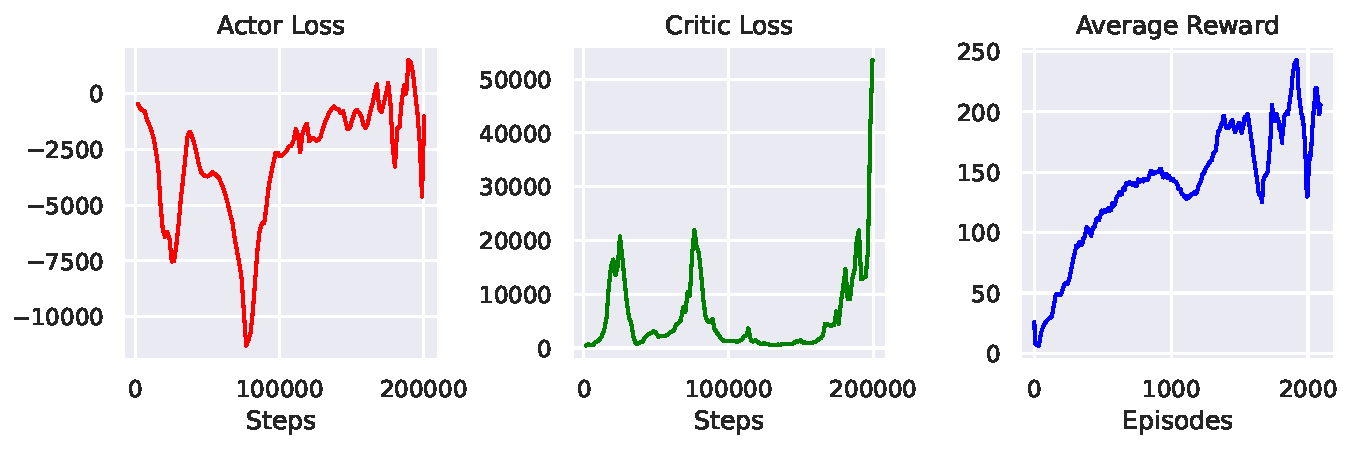
\includegraphics[width=\linewidth]{images/exp-hopper-tau0.05.pdf}
  \caption{$\tau = 0.05$.}
\end{figure*}

\begin{figure*}[ht]
  \centering
  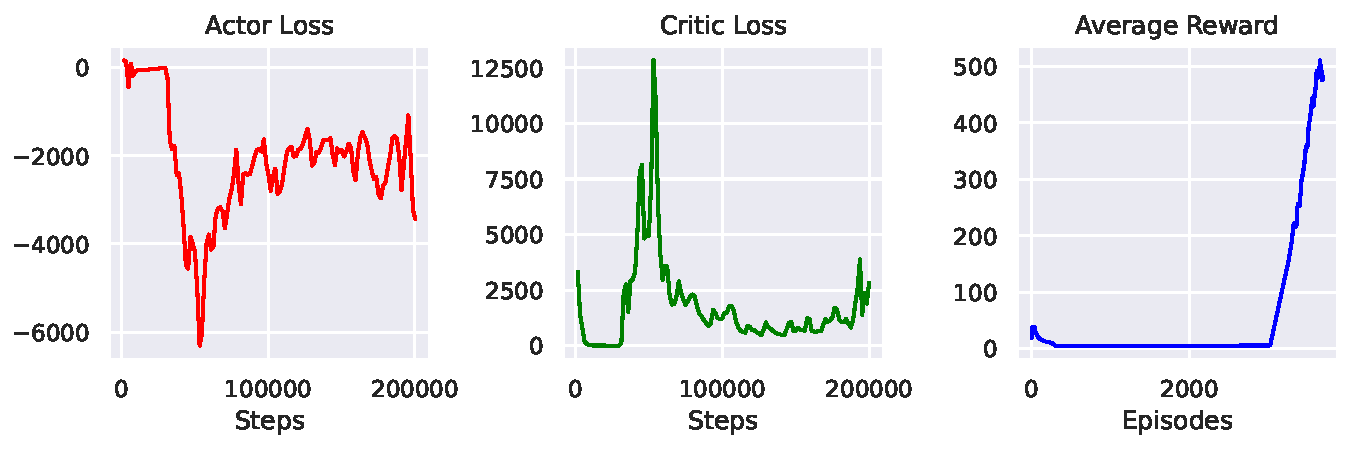
\includegraphics[width=\linewidth]{images/exp-hopper-tau0.1.pdf}
  \caption{$\tau = 0.1$.}
   \label{fig:boom}
\end{figure*}

\begin{figure*}[ht]
  \centering
  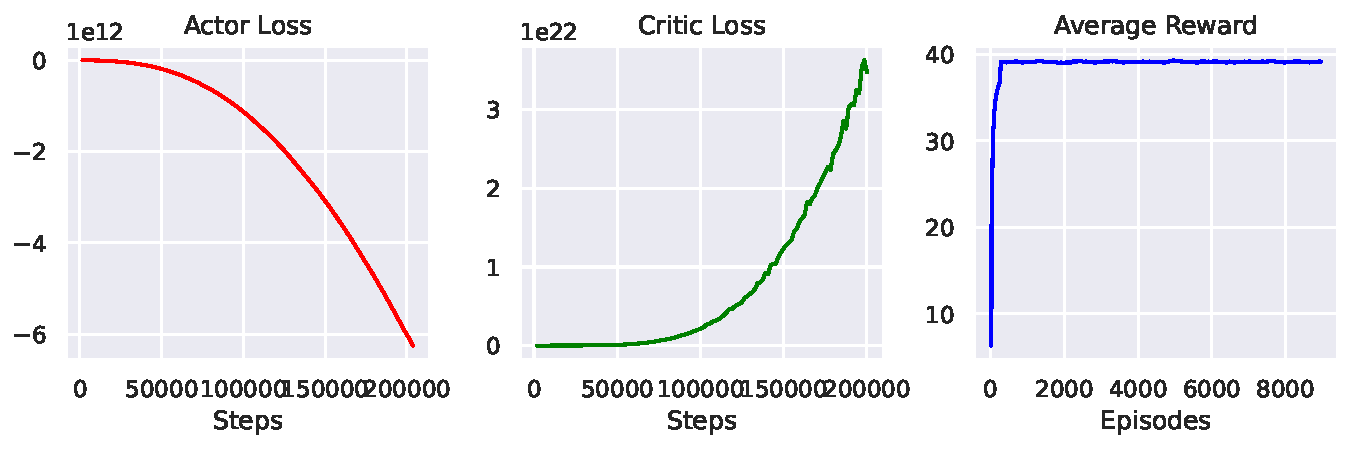
\includegraphics[width=\linewidth]{images/exp-hopper-tau0.4.pdf}
  \caption{$\tau = 0.4$.}
\end{figure*}

\begin{figure*}[ht]
  \centering
  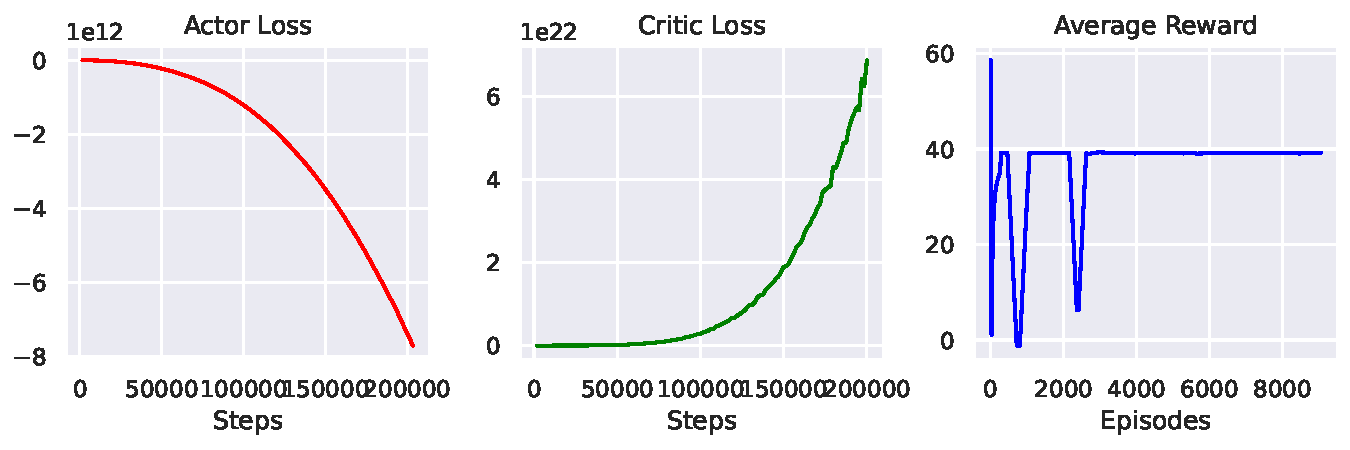
\includegraphics[width=\linewidth]{images/exp-hopper-tau0.8.pdf}
  \caption{$\tau = 0.8$.}
\end{figure*}

\begin{figure*}[ht]
  \centering
  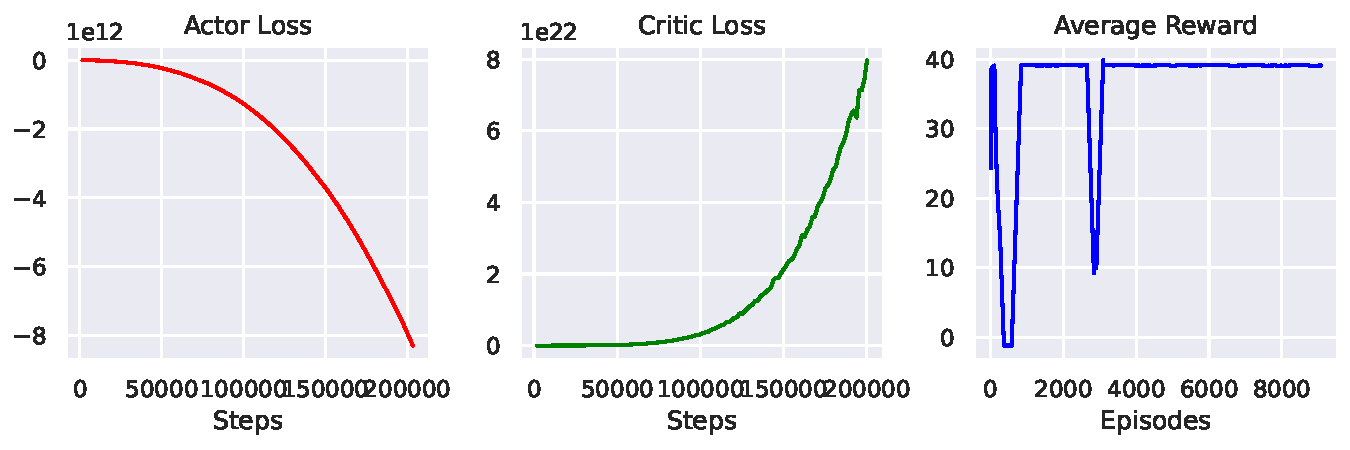
\includegraphics[width=\linewidth]{images/exp-hopper-tau1.pdf}
  \caption{$\tau = 1.0$.}
\end{figure*}

\else
    % \input{2019-PPFIT-ShortName-text-en.tex}
\fi

%--------------------------------------------------------
%--------------------------------------------------------
%--------------------------------------------------------
%	LITERATURA
%--------------------------------------------------------
%--------------------------------------------------------
\phantomsection
\ifczech
    \bibliographystyle{bib-styles/czplain}
\fi
\ifslovak
    \bibliographystyle{bib-styles/skplain}
\fi
\ifenglish
    \bibliographystyle{bib-styles/enplain}
\fi

\bibliography{doc-bib}

%--------------------------------------------------------
%--------------------------------------------------------
%--------------------------------------------------------

\end{document}